\documentclass[aspectratio=169]{beamer}
\usepackage{babel}
% \usepackage[german]{babel}

\usepackage{tikz, transparent, colortbl, listings, pgfplots}
\usepackage[export]{adjustbox}
\usepackage[skins,theorems]{tcolorbox}
 
\usetikzlibrary{automata,positioning}
\setbeamercovered{transparent}
\pgfplotsset{compat=1.18}
\tcbset{highlight math style={enhanced,colframe=red,colback=white,arc=0pt,boxrule=1pt}}

%
% Cited from Ausarbeitung/aspdoc.cls
%
\lstset{
    language=C++,
    basicstyle=\upshape\footnotesize\ttfamily,
    numbers=left,                   % where to put the line-numbers
    numberstyle=\tiny\color{gray},  % the style that is used for the line-numbers
    numbersep=5pt,                  % how far the line-numbers are from the code
    showstringspaces=false,
    frame=single,                   % adds a frame around the code
    rulecolor=\color{black},
    tabsize=2,                      % sets default tabsize to 2 spaces
    captionpos=b,                   % sets the caption-position to bottom
    breaklines=true,                % sets automatic line breaking
    breakatwhitespace=false,        % sets if automatic breaks should only happen at whitespace
    title=\lstname,                 % show the filename of files included with \lstinputlisting;
    keywordstyle=\color{blue},      % keyword style
    commentstyle=\color{dkgreen},   % comment style
    stringstyle=\color{mauve},      % string literal style
    escapeinside={\%*}{*)},         % if you want to add LaTeX within your code
}

% Useful Read:
% https://www.overleaf.com/learn/latex/Beamer

\title{Molecular Dynamics}
\subtitle{Group A}
\author{Haoyuan Ma \and Zhengying Zhao \and Anatoly Weinstein}
\date{31st of October 2025}

\newcommand{\framebackground}[2]{
    \begin{tikzpicture}
        \transparent{#1}
        \node[inner sep=0] at (current page.center) {
            
\includegraphics[height=\paperheight, right]{./media/tum-uhrenturm.png}
        };
        \transparent{1}
        \node[anchor=south, text width=\paperwidth, text height=1.5cm, draw=none, align=center] at (current page.south) {
            \insertpagenumber
        };
        \transparent{#2}
        \node[anchor=south, text width=\paperwidth, text height=1.5cm, draw=none, align=right] at (current page.south) {
            \small Haoyuan Ma, Zhengying Z, Anatoly W. \,\,
        };
    \end{tikzpicture}
}

\newcommand{\headerframe}{
    \usebackgroundtemplate{
        \framebackground{0.2}{1}
    }
}

\newcommand{\simpleframe}{
    \usebackgroundtemplate{
        \framebackground{0}{1}
    }
}

\newcommand{\blue}[1]{{\color{beamer@blendedblue} #1}}
\newcommand{\yellow}[1]{{\color[HTML]{AF8F10} #1}}
\newcommand{\gray}[1]{{\color[HTML]{8F8F8F} #1}}
\newcommand{\red}[1]{{\color[HTML]{FF5F5F} #1}}

\begin{document}

%
% Frame
%
\usebackgroundtemplate{\framebackground{0.2}{0}}
\begin{frame}
    \maketitle
\end{frame}

\simpleframe\begin{frame}{Github CI: Checks Passed}
    \centering
    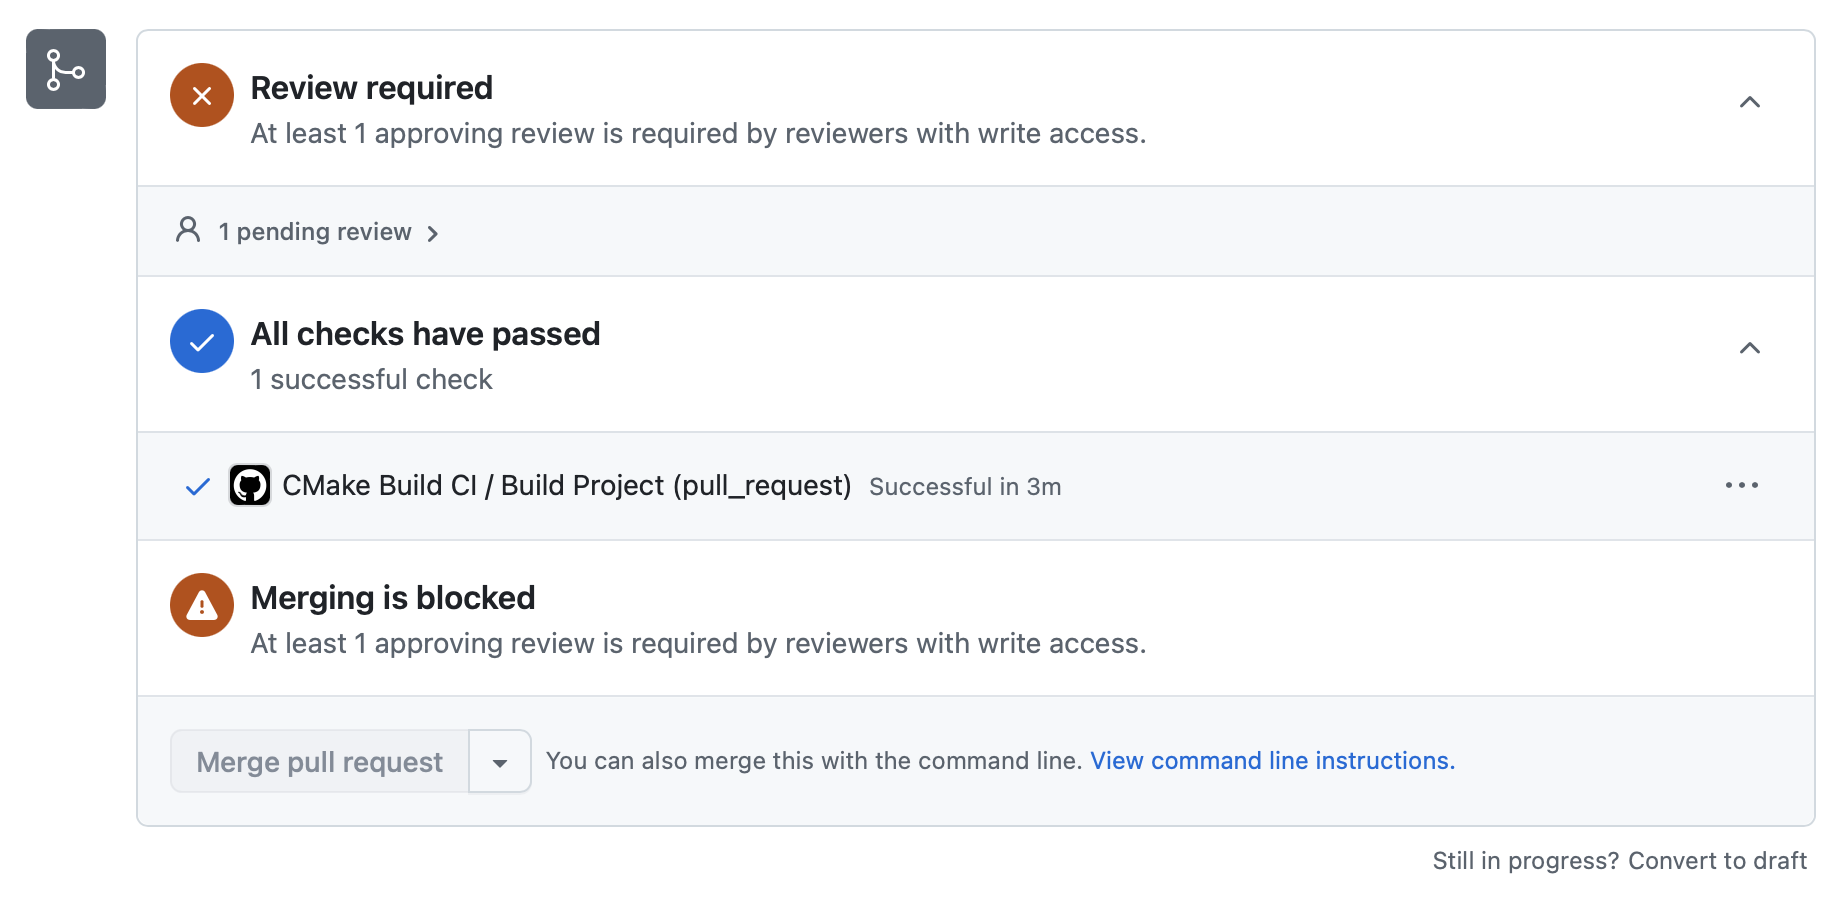
\includegraphics[width=0.95\textwidth]{media/github_checks.png}
\end{frame}

\simpleframe\begin{frame}{Github Rulesets}
    \begin{itemize}
        \item Two rulesets: \blue{Block Push Master} and \blue{Block Push Assignments}
        \item Require Pull Requests to merge: E.g.: \texttt{a2/task2} into \texttt{assignment2}, then \texttt{assignment2} into \texttt{master} $\rightarrow$ Everyone works in their dedicated branches.
        \item Pull Requests to \texttt{master} requires approval $\rightarrow$ Enhanced Protection
        \item \alert{Block Force Pushes!}
    \end{itemize}
\end{frame}


\simpleframe\begin{frame}[fragile]{Benchmarking: Our Algorithm is Bad}

    \begin{columns}
        \begin{column}{0.5\textwidth}
            \texttt{eingabe-sonne.txt}

% Benchmark Iteration 0: 0.089082s
% Benchmark Iteration 1: 0.07885s
% Benchmark Iteration 2: 0.073647s
% Benchmark Iteration 3: 0.072196s
% Benchmark Iteration 4: 0.072877s
% Benchmark Iteration 5: 0.073609s
% Benchmark Iteration 6: 0.071922s
% Benchmark Iteration 7: 0.078932s
% Benchmark Iteration 8: 0.077366s
% Benchmark Iteration 9: 0.075796s
% Average Duration over 10 iterations, over 4 particles: 0.0764277s
            \begin{lstlisting}
Benchmark Iteration 0: 0.09268s
Benchmark Iteration 1: 0.082871s
Benchmark Iteration 2: 0.102149s
Benchmark Iteration 3: 0.110204s
Benchmark Iteration 4: 0.082761s
Average Duration over 5 iterations, over 4 particles: 0.094133s
            \end{lstlisting}
            \vspace{-1.5em}
            4 particles in $\leq$ 0.1s
        \end{column}
        \begin{column}{0.5\textwidth}
            \texttt{shaw.txt}
% Benchmark Iteration 0: 14.0857s
% Benchmark Iteration 1: 13.5396s
% Benchmark Iteration 2: 13.204s
% Benchmark Iteration 3: 12.547s
% Benchmark Iteration 4: 21.4599s
% Benchmark Iteration 5: 20.3371s
% Benchmark Iteration 6: 22.8944s
% Benchmark Iteration 7: 19.1164s
% Benchmark Iteration 8: 19.1016s
% Benchmark Iteration 9: 15.285s
% Average Duration over 10 iterations, over 58 particles: 17.1571s
            \begin{lstlisting}
Benchmark Iteration 0: 14.8056s
Benchmark Iteration 1: 21.1189s
Benchmark Iteration 2: 17.3226s
Benchmark Iteration 3: 16.7992s
Benchmark Iteration 4: 12.6689s
Average Duration over 5 iterations, over 58 particles: 16.543s
            \end{lstlisting}
            \vspace{-1.5em}
            58 particles in 17s
        \end{column}
    \end{columns}

    \vspace{1.5em}

    \alert{Unacceptable runtime!} Right now we can not afford to simulate hundreds or thousands of particles.
\end{frame}

\simpleframe\begin{frame}[fragile]{Benchmarking: Better, But still pretty Bad}

    \begin{columns}
        \begin{column}{0.5\textwidth}
            \texttt{eingabe-sonne.txt}
            \begin{lstlisting}
Benchmark Iteration 0: 0.058703s
Benchmark Iteration 1: 0.053112s
Benchmark Iteration 2: 0.050419s
Benchmark Iteration 3: 0.048694s
Benchmark Iteration 4: 0.048469s
Average Duration over 5 iterations, over 4 particles: 0.0518794s
            \end{lstlisting}
            \vspace{-1.5em}
            4 particles in $\sim$ 0.05s \gray{previously: 0.10s}
        \end{column}
        \begin{column}{0.5\textwidth}
            \texttt{shaw.txt}
            \begin{lstlisting}
Benchmark Iteration 0: 9.58458s
Benchmark Iteration 1: 7.43857s
Benchmark Iteration 2: 7.69406s
Benchmark Iteration 3: 7.52219s
Benchmark Iteration 4: 7.37951s
Average Duration over 5 iterations, over 58 particles: 7.92378s
            \end{lstlisting}
            \vspace{-1.5em}
            58 particles in 8s \gray{previously: 17s}
        \end{column}
    \end{columns}

    \vspace{1.5em}

    Iteration over distinct pairs \blue{(applying Newtons' 3rd law) doubles performance}, but the problem lies in the algorithm.
\end{frame}

\headerframe\begin{frame}{That's it – for now, at least}{Shaw! We thank you for your attention!}
    \begin{center}
        \begin{figure}
        \centering
        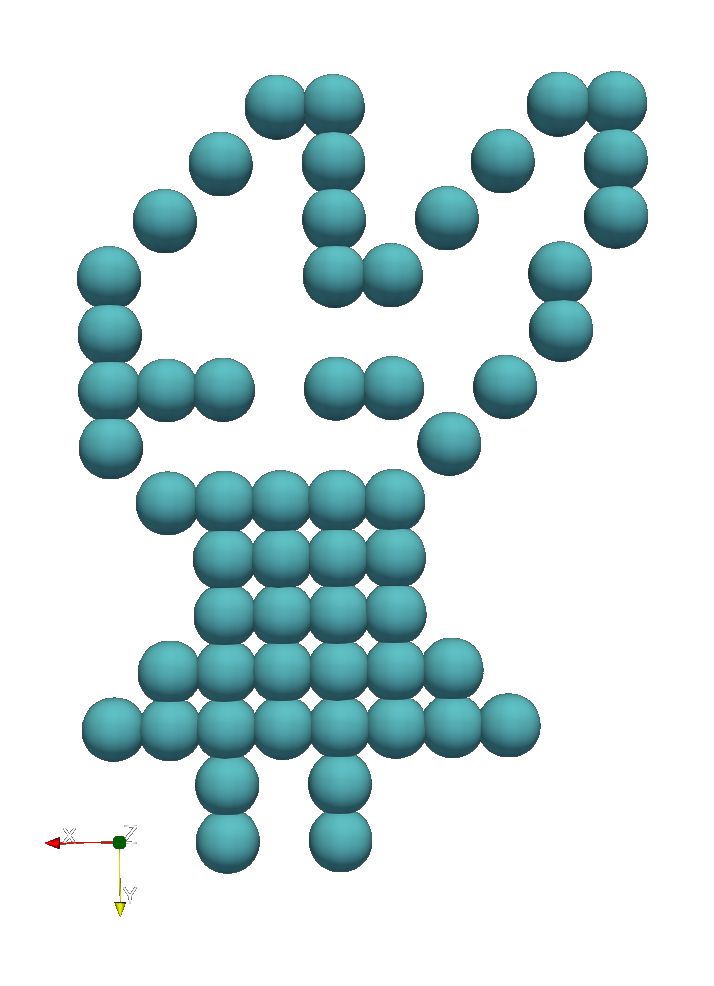
\includegraphics[width=0.35\textwidth]{media/shaw.png}
    \end{figure}
    \end{center}
\end{frame}

\end{document}
